\subsection{Reinforcement Learning}

In this section, I describe concepts from reinforcement learning as they will be used in the proposed research.  Reinforcement learning is a sub field of artificial intelligence used in optimal decision making. The term "reinforcement" indicates that the algorithms learn from actions which are rewarded, with favourable actions being rewarded according to their benefit \cite{sutton2011reinforcement}.  Thus, the algorithms learn through positive/negative "reinforcement".  The actions and their reward are not typically know \textit{a priori}, and so these algorithms are said to "learn from experience".  In particular, sequential decision making,Markov decision processes, and optimal policies, and goals for learning algorithms are discussed.

\subsubsection{Formalization of Sequential Decision Making}

Reinforcement learning idealizes the algorithm (or entity doing the decision making) as an \textit{agent} continually interacting with a \textit{environment}.  At a sequence of discrete time steps  (${ t =1, 2 \dots, n} $), the agent evaluates the current \textit{state} of the environment $ S_t $, decides on an \textit{action} ($ A_t $), receives a \textit{reward} for that action $ R_{t+1} $, and then finds itself in a \textit{new state} ($ S_{t+1} $).  This sequence of state, action, reward, new state is called a \textit{trajectory} \cite{sutton2011reinforcement,lizotte2017reinforcement}.  Here, 

The set of all states in which the agent may find itself in ($\mathcal{S}$), the set of all actions which the agent may make ($\mathcal{A}$), the set of rewards given to the agent ($ \mathcal{R} $), and the distribution of new states ($ P $) the agent could find itself in if it takes action $ a_t $ in stats $ s_t $ for a \textit{Markov decision process} (MPD) \cite{sutton2011reinforcement,lizotte2017reinforcement}.

\begin{figure}[h!]
\centering
	
\tikzstyle{block} = [rectangle, draw, 
text width=8em, text centered, rounded corners, minimum height=4em]

\tikzstyle{line} = [draw, -latex]
\tikzstyle{block} = [rectangle, draw, 
text width=8em, text centered, rounded corners, minimum height=4em]

\tikzstyle{line} = [draw, -latex]

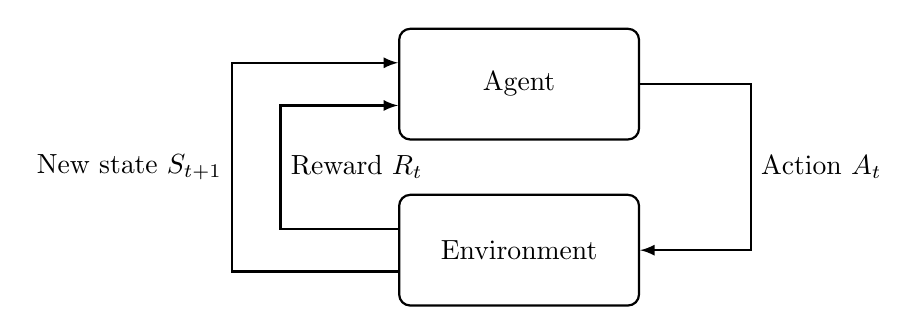
\begin{tikzpicture}[node distance = 6em, auto, thick]
\node [block] (Agent) {Agent};
\node [block, below of=Agent] (Environment) {Environment};

\path [line] (Agent.0) --++ (4em,0em) |- node [near start]{Action $A_t$} (Environment.0);
\path [line] (Environment.190) --++ (-6em,0em) |- node [near start] {New state  $S_{t+1}$} (Agent.170);
\path [line] (Environment.170) --++ (-4.25em,0em) |- node [near start, right] {Reward $R_{t}$} (Agent.190);
\end{tikzpicture}

\caption[Reinforcement learning process]{Pictorial representation of the learning process.  At the present state $ S_t $, the agent makes action $ A_t $.  The action is rewarded with $ R_t $ and the agent finds itself in a new state $ S_{t+1} $.  The process repeats and forms a trajectory of $ {S_t,A_t,R_t,S_{t+1}, A_{t+1}, R_{t+1}, S_{t+2}, \cdots} $.  }
\label{RL_diagram}
\end{figure}


\subsubsection{Policies}

The agent will choose actions based on a \textit{policy}.  A policy, $ \pi $, is a function which maps the set of states to the set of actions  
%
\begin{equation}\label{key}
\pi : \mathcal{S} \rightarrow \mathcal{A}\>.
\end{equation}
%
Associated with a particular trajectory is a \textit{return}, $ \sum_t R_t \gamma^t $, where $ \gamma $ is constant and $ 0 < \gamma < 1 $.  The environment is assumed to be stochastic, thus the return are random quantities. Let $ \mathbf{\Psi}_{\pi,s} $ be a random variable for the return following policy $ \pi $ in state $ s $.  The \textit{value} of a policy is the expected return of that policy, $V_{\pi}(s) =  \mathbb{E}(\mathbf{\Psi}_{\pi,s}) $ \cite{lizotte2017reinforcement}.  A policy is said to be \textit{optimal} if the value of the policy is larger than all other policies under all possible states.  Mathematically, a policy $ \pi^* $ is optimal if and only if $ V_{\pi}(s)  \leq V_{\pi^*}(s) \> \forall \pi, \forall s\in \mathcal{S}  $.


\subsubsection{Goals for Learning}
Different algorithms seek to learn different aspects of the problem at hand.  Temporal difference learning seeks to compute a value function given by experience generated by a policy, while Q-learning attempts to learn an optimal policy given the agent's experience \cite{lizotte2017reinforcement}.  The details of these algorithms are beyond the scope of this proposal.